\section{Мова програмування С++}
\Authors{\textbf{Овсянніков Олександр Сергійович}}
\Address{}{\href{mailto:vinniaso@gmail.com}{vinniaso@gmail.com}}

\begin{wrapfigure}{L}{0.25\textwidth}
	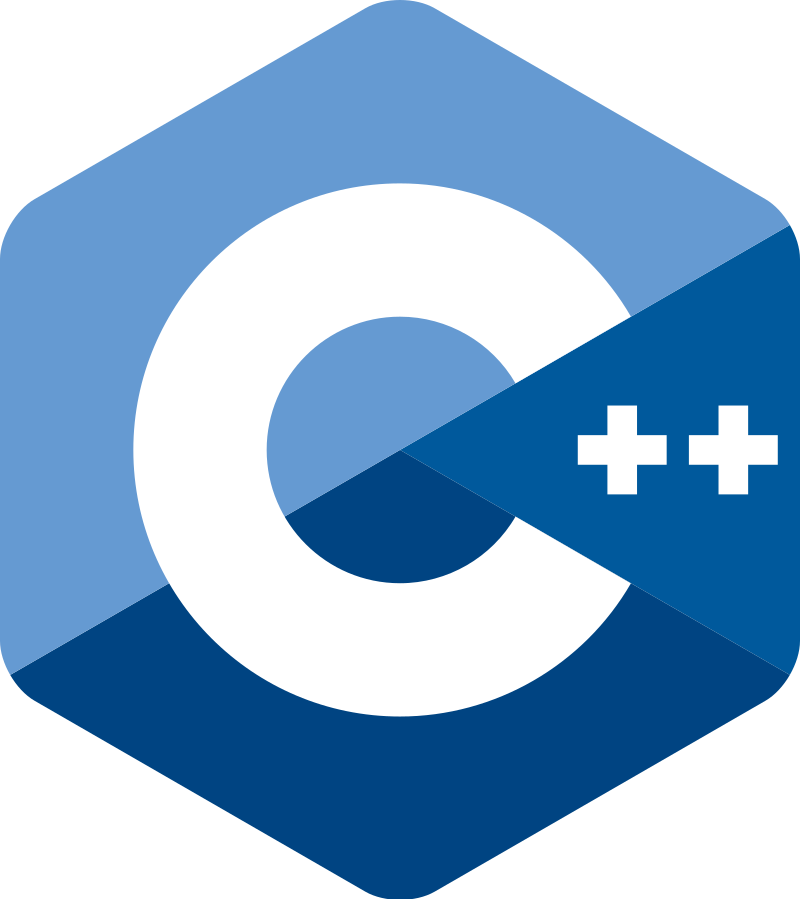
\includegraphics[width=3cm]{ISO_C++_Logo.svg.png}\\
	\caption{\label{fig:frog1} Логотип.}
\end{wrapfigure} 
\textbf{Мова програмування С++} представляє собою високорівневу мову програмування загального призначення зі статичною типізацією, що підходить для створення найрізноманітніших програмних продуктів. На сьогоднішній день С++ є однією з найпопулярніших (див. \href{https://www.tiobe.com/tiobe-index/}{TIOBE Index}) та найпоширеніших мов програмування.
Мова C++ є еволюційним розвитком мови програмування C. Мова C була розроблена на початку 1970-х років в Bell Labs під час розробки операційної системи Unix. Автором мови C вважається \href{https://uk.wikipedia.org/wiki/%D0%94%D0%B5%D0%BD%D0%BD%D1%96%D1%81_%D0%A0%D1%96%D1%82%D1%87%D1%96}{Денніс Рітчі} (\textit{Dennis Ritchie}), якому не вистачало доступних на той момент інструментів мов програмування для написання коду операційної системи Unix. На початку 1980-х років датський програміст \href{https://uk.wikipedia.org/wiki/%D0%91%27%D1%8F%D1%80%D0%BD_%D0%A1%D1%82%D1%80%D0%B0%D1%83%D1%81%D1%82%D1%80%D1%83%D0%BF}{Б’ярн Страуструп} (\textit{Bjarne Stroustrup}), який на той час працював у компанії Bell Labs, розробив мову С++ як розширення до мови програмування С. Фактично спочатку мова C++ просто доповнювала мову С деякими можливостями об'єктно-орієнтованого програмування. І тому, сам Страуструп спочатку називав мову – «С з класами» (\textit{«C with classes»}). Згодом нова мова програмування стала набирати популярності. До неї були додані нові можливості, які робили її не просто доповненням до мови С, а й взагалі новою мовою програмування. У результаті в 1983 році мову програмування «С з класами» було перейменовано на С++. І з тих пір обидві мови програмування стали розвиватися незалежно одна від одної.

\begin{center}
	\textbf{Історія версій}
\end{center}
\begin{longtable}{| p{.1\textwidth} | p{0.8\textwidth} |} 
	\hline
	1985 & випущена перша комерційна версія мови С++, а також перше видання книги «Мова програмування C++», яка представляла перший опис цієї мови за відсутності офіційного стандарту \\ \hline 
	1989 & випущена нова версія мови C++ 2.0, що включала низку нових можливостей \\ \hline
	1998 & була зроблена перша спроба стандартизації цієї мови програмування організацією \href{https://uk.wikipedia.org/wiki/%D0%9C%D1%96%D0%B6%D0%BD%D0%B0%D1%80%D0%BE%D0%B4%D0%BD%D0%B0_%D0%BE%D1%80%D0%B3%D0%B0%D0%BD%D1%96%D0%B7%D0%B0%D1%86%D1%96%D1%8F_%D0%B7%D1%96_%D1%81%D1%82%D0%B0%D0%BD%D0%B4%D0%B0%D1%80%D1%82%D0%B8%D0%B7%D0%B0%D1%86%D1%96%D1%97}{International Organiztion for Standartization} (ISO). Перший стандарт отримав назву ISO/IEC 14882:1998 або скорочено C++98 \\ \hline
	2003 & було видано нову версію стандарту C++03 \\ \hline
	2011 & видано новий стандарт C++11, який містив безліч додавань та збагачував мову програмування С++ великою кількістю нових функціональних можливостей \\ \hline
	2014 & було випущено невелике додавання до стандарту, відоме також, як C++14 \\ \hline
	2017 & cтандарт С++17 був офіційно опублікований. Було внесено ряд змін в мову програмування, зокрема додано декілька нових бібліотек, алгоритмів  та класів до стандартної бібліотеки шаблонів (STL), поліпшено роботу з лямбда-виразами, оновлено бібліотеку <thread> для мультипотокового програмування \\ \hline
	2020 & cтандарт C++20. Ця версія має набагато більше нововведень в порівнянні з C++14 та C++17. Зокрема, ця версія вводить «концепції», «співпрограми», новий оператор порівняння <=>, тощо \\ \hline
\end{longtable}

\textbf{С++} є потужною мовою програмування, яка успадкувала від мови С багато можливостей по роботі з пам'яттю. Тому нерідко мова С++ знаходить своє застосування у системному програмуванні, зокрема, при створенні операційних систем, драйверів, різних утиліт, антивірусів тощо. До речі, ОС Windows переважно написана на мові програмування С++. Але лише системним програмуванням застосування цієї мови не обмежується. 

\textbf{С++} можна використовувати у програмах будь-якого рівня, де важливі швидкість роботи та продуктивність. Нерідко вона застосовується для створення графічних додатків, різних прикладних програм. Також особливо часто її використовують для створення ігор із насиченою візуалізацією. Крім того, мова С++ застосовується в мобільному програмування, у веб-розробці для створення веб-додатків або будь-яких допоміжних сервісів, які обслуговують веб-додатки. Загалом С++ – мова програмування широкого користування, якою можна створювати практично будь-які види програмного забезпечення.

